% - ``Upper-Confidence Bound for Channel Selection in LPWA Networks with Retransmissions'', see  https://hal.inria.fr/hal-02049824

\graphicspath{{2-Chapters/4-Chapter/IEEE_WCNC__2019__Paper__BMBM.git/}}


% In the context of Cognitive Radio \cite{Mitola99,Haykin05},
% Multi-Arm Bandit (MAB) algorithms \cite{Auer02,Auer02,Bubeck12} have been recently proposed as a potential solution for channel access in LPWA networks \cite{Bonnefoi18,Azari18,Bonnefoi17}.
We presented in Section~\ref{sec:4:firstModel} low-cost algorithms following well-known approaches, such as Upper-Confidence Bound (\UCB), and we have reported encouraging results.
When considering the application of MAB algorithms for slotted wireless protocols in a decentralized manner,
other recent directions of research include theoretical analysis, like what we present in the next Chapter~\ref{chapter:5},
or realistic empirical PoC like in \cite{RobertSDR2014,modiDemo2016,darak2016bayesian,kumar2017channel} or the previous Section~\ref{sec:4:gnuradio},
and finally applications to multi-hoping networks \cite{Mitton16,Toldov16} or other kinds of networks \cite{Azari18,Wilhelmi19collaborative,Wilhelmi19potential}.
%
None of the mentioned works discuss the impact of retransmissions on the performance of MAB learning algorithms.

In this section, we extend the previous model to take into account the possibility for retransmissions of a message after a collision.
This is of major importance as most protocols for real-world IoT networks can use retransmissions, it is for instance the case of the LoRaWAN standard \cite{Raza17}.
As before, we propose and evaluate different learning strategies based on MAB algorithms.
However, the price to be paid is a shorter battery lifetime for IoT devices. So this approach would be used only for devices with strong delivery constraints (\eg, for health-care applications), or that can refuel their energy over time (\eg, for robotic applications).

% The presented strategies allow IoT devices to improve their access to the network and their autonomy, while taking into account the impact of encountered radio collisions.
% For that end, several heuristics employing \UCB{} algorithms are examined, to explore the information provided by the number of retransmissions.
% In this section, our results show that approaches based on \UCB{} obtain a significant improvement in terms of successful transmission probabilities, compared to a naive approach which does not learn.
% Furthermore, it also reveals that a pure \UCB{} channel access is as efficient as more sophisticated learning strategies.

% \TODOL{This section is based on the publication ``Upper-Confidence Bound for Channel Selection in LPWA Networks with Retransmissions'', see \texttt{https://hal.inria.fr/hal-02049824}}

% https://hal.inria.fr/hal-02049824


% % ----------------------------------------------------------------------
% \subsection{Retransmissions in an ALOHA like protocol}
% \label{sub:43:introduction}
% % ----------------------------------------------------------------------

We want to assess the performance of MAB algorithms for channel selection in LPWA networks operating in unlicensed bands, while taking into account the impact of retransmissions on the network performance.
For this reason, several decision making strategies are applied after a first retransmission (\ie, when a collision occurs).
The proposed approach employs contextual information provided by the number of retransmissions, and is again implemented independently by each device, so that no coordination among them is needed.
Moreover, our \UCB{}-based heuristics again show low complexity, which make them suitable for being embedded in LPWA devices, like in the previous sections.

The contributions of this section can be thus summarized as follows.
% \begin{itemize}
	% \item
	Firstly, we provide a close form approximation of the radio collision probability after a first retransmission.
	By doing this, we highlight the need to develop a learning approach for channel selection upon collision.
%
	% \item
	Secondly, different heuristics are proposed to cope with retransmissions.
%
	% \item
	Lastly, we conduct simulations in order to compare the performance of the proposed heuristics with a naive uniform random approach, and a \UCB{} strategy (\ie, without any learning for the retransmissions, that is, the same channel is used for retransmission).
% \end{itemize}


% \textbf{Outline.}
% %
% The rest of the section is organized as follows.
% First the system model is introduced in Section~\ref{sub:43:model},
% and our motivations are exposed in Section~\ref{sub:43:motivations}.
% The proposed \UCB-based heuristics are presented in Section~\ref{sub:43:heuristics}, while the corresponding numerical results are shown in Section~\ref{sub:43:numExp}.
% Finally, some conclusions are drawn later in Section~\ref{sub:43:conclusion}.


% ----------------------------------------------------------------------
% \subsection{Extending our model with retransmissions}
\subsection{Presentation of the model with retransmissions}
\label{sub:43:model}
% ----------------------------------------------------------------------

% ----------------------------------------------------------------------
\paragraph{LPWA network.}

Like in the previous sections of this chapter, we consider an LPWA network \cite{Raza17}, composed of a gateway and a large number of end-devices that regularly send short data packets, where $K$ channels ($K>1$) are available for the transmission of their packets.
%
We assume that this network is constituted by two types of devices:
On the one hand, we have \emph{static} devices that operate in one channel\footnote{~Note that, for unlicensed bands, this definition also encompasses any device following a different standard or trying to establish communication with gateways of other networks.} in order to communicate with the gateway.
%
On the other hand, there are  IoT devices, that possess the additional advantage of being able to select any of the $K$ available channels to perform their transmissions.

Like in the previous model presented in Section~\ref{sec:4:firstModel},
regardless the type of devices, each of them follows a slotted ALOHA protocol \cite{Roberts75}, and has a probability $p>0$ to transmit a packet in a time slot.
We make the hypothesis that the transmission is successful if the channel is available, otherwise it fails upon radio collision.
The novelty compare to the previous model is that
in case of RF (uplink or downlink) collision that prevent the device to receive the \emph{Ack} from the gateway,
these devices will attempt to retransmit their packet up-to $\mathrm{MaxBackOff}$ times\footnote{~We denote it $\mathrm{MaxBackOff}$ instead of $M$ like we did in our paper \cite{Bonnefoi2019WCNC}, as $M$ is used in next Chapter~\ref{chapter:5}.},
with $\mathrm{MaxBackOff} \in\mathbb{N}^*$.
It is important to note that, every retransmission is carried out after a random back-off time, uniformly distributed in $\{0, \dots, m-1\}$, where $m \in\mathbb{N}^*$ is the length of the back-off interval
(note the difference between $m$ and $\mathrm{MaxBackOff}$).


% ----------------------------------------------------------------------
\paragraph{Model of IoT devices.}

The aforementioned contention process can be described by a Markov chain model \cite{Norris98} similar to the one presented in \cite{Yang12}, as it is depicted in Figure~\ref{fig:43:Markov_model}.
When a device has a packet to transmit, it goes from an idle state to a transmission state, while considering retransmissions due to different collision probabilities, $p_{c}, p_{c1}, \dots, p_{c\mathrm{MaxBackOff}-2}$, at each $\mathrm{MaxBackOff}$ back-off stage.
At each time slot, a transition from an idle state to a transmission state (denoted as \texttt{Trans.}) occurs if a packet transmission is required, while waiting states (denoted as \texttt{Wait}), correspond to a $m$ back-off interval.

\begin{figure}[!h]
	\centering
	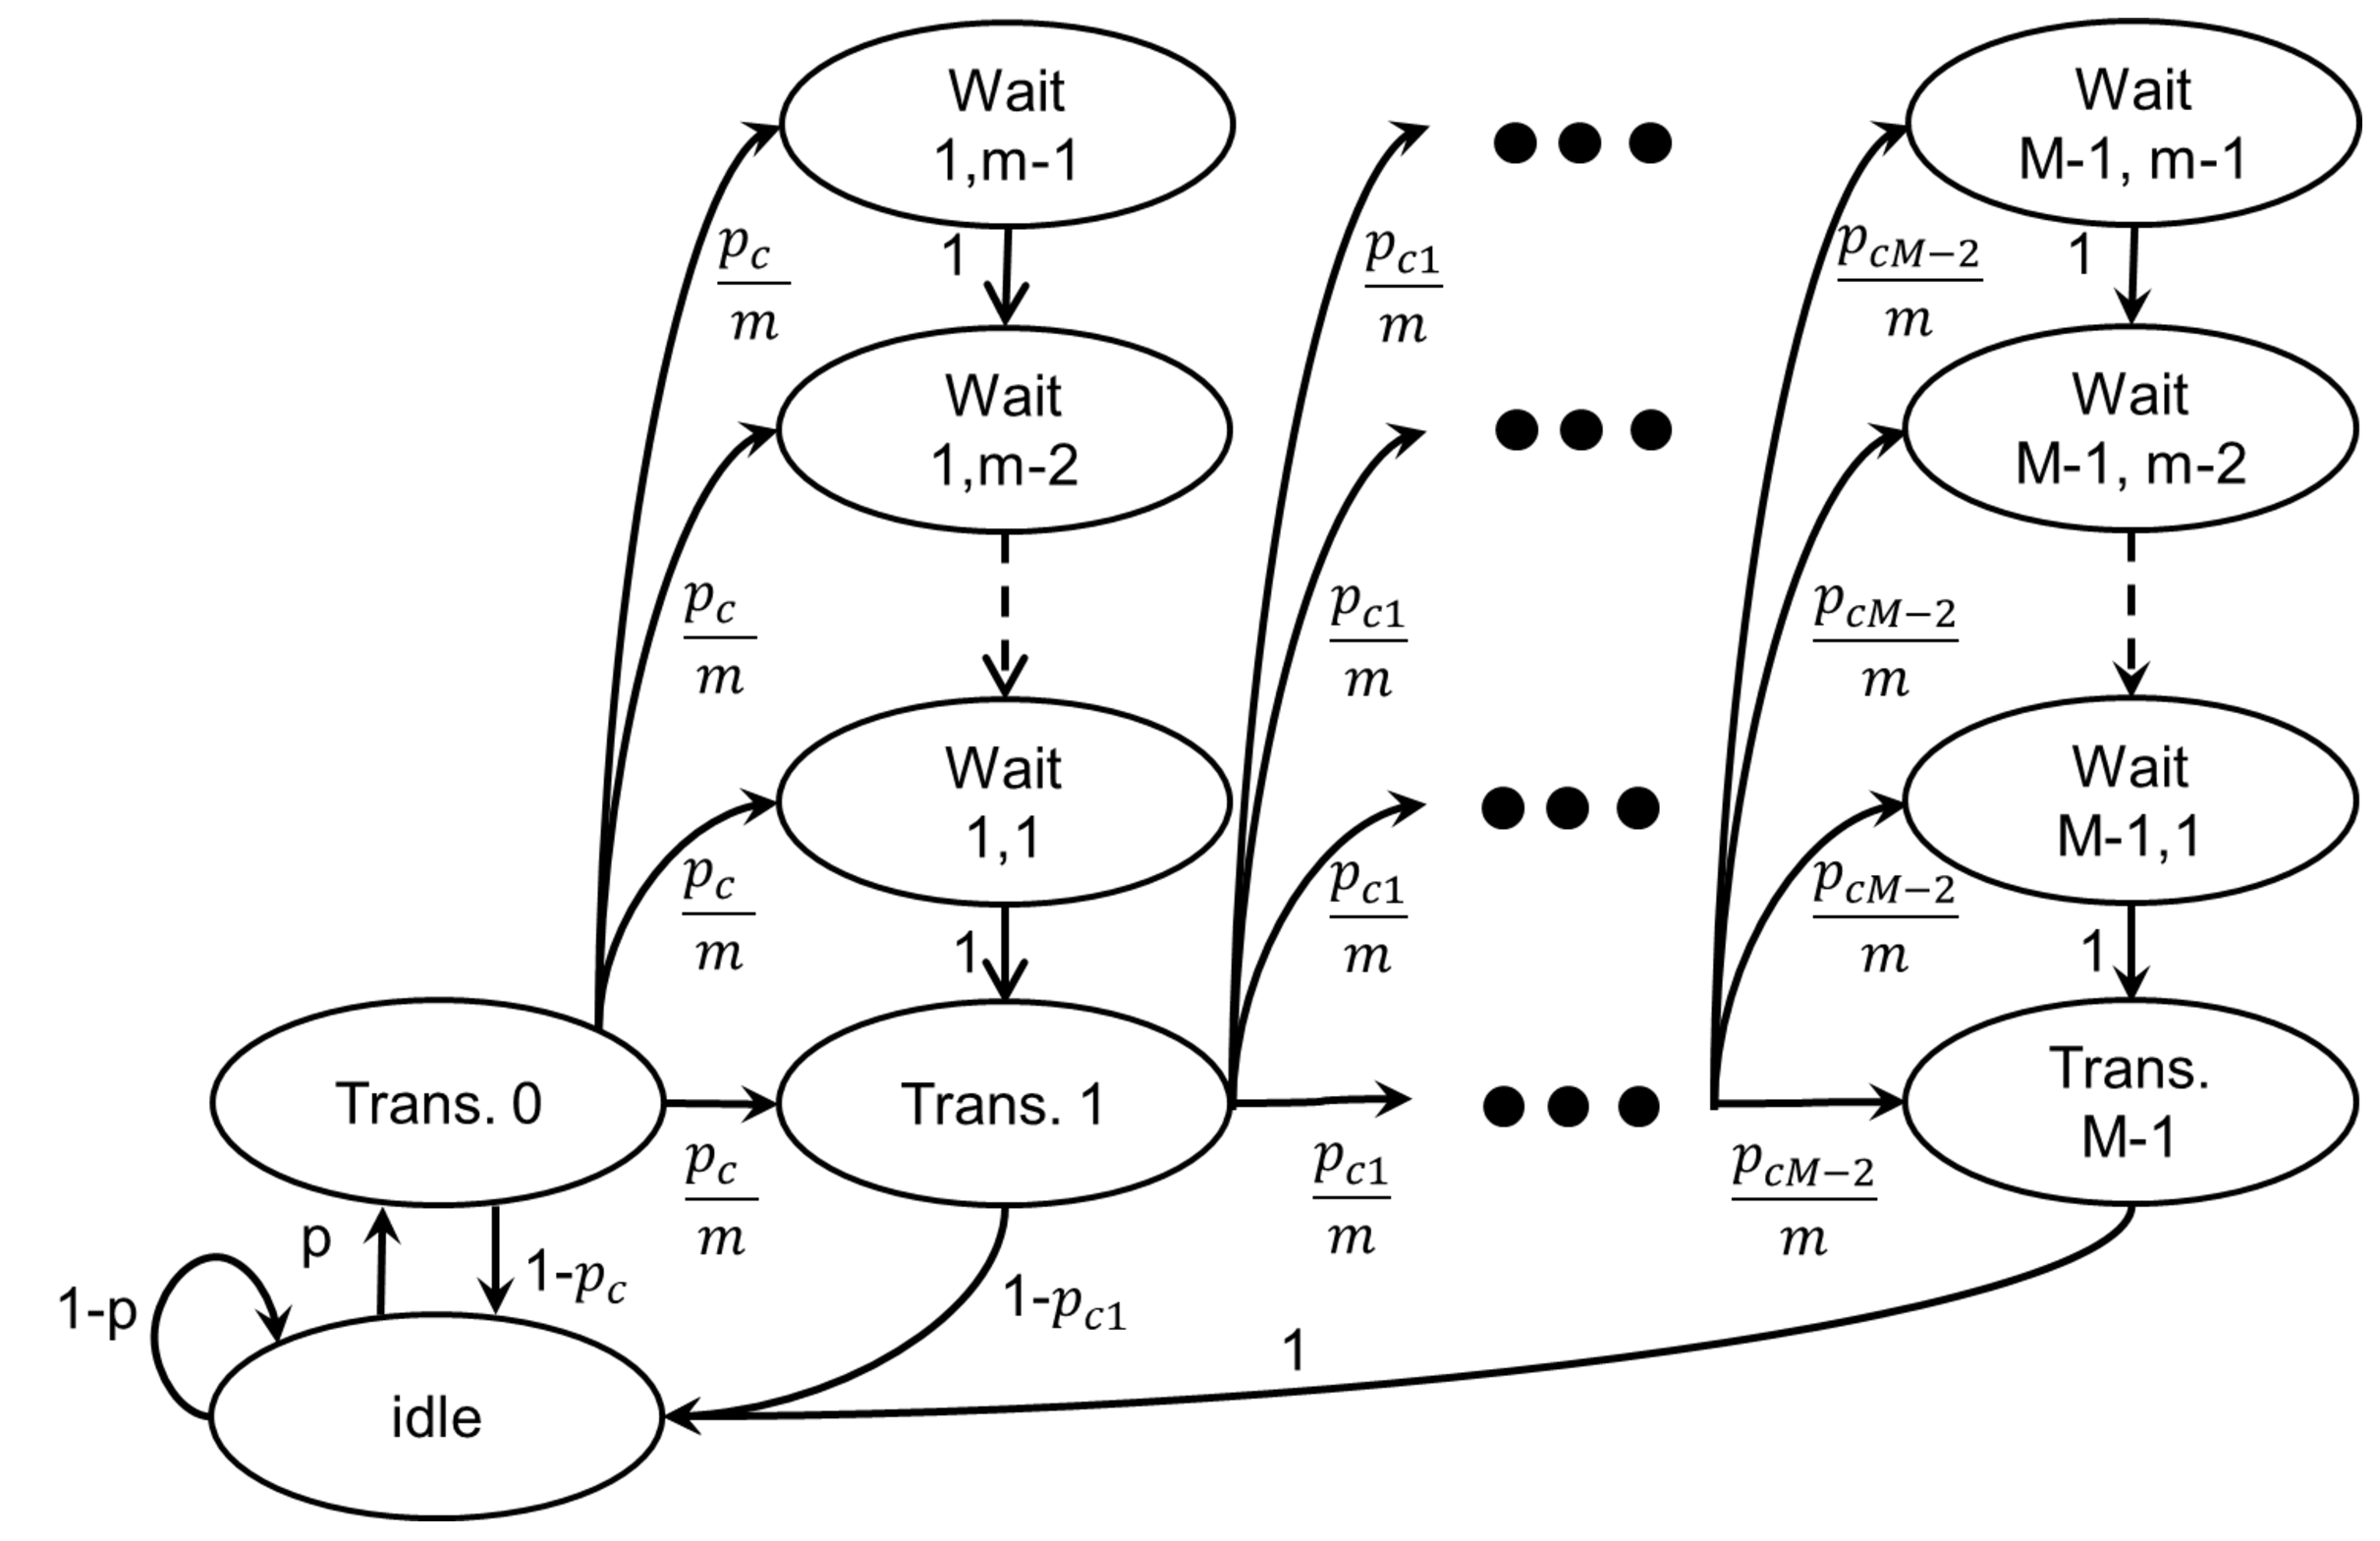
\includegraphics[width=0.70\linewidth]{Markov_model.eps}
	% 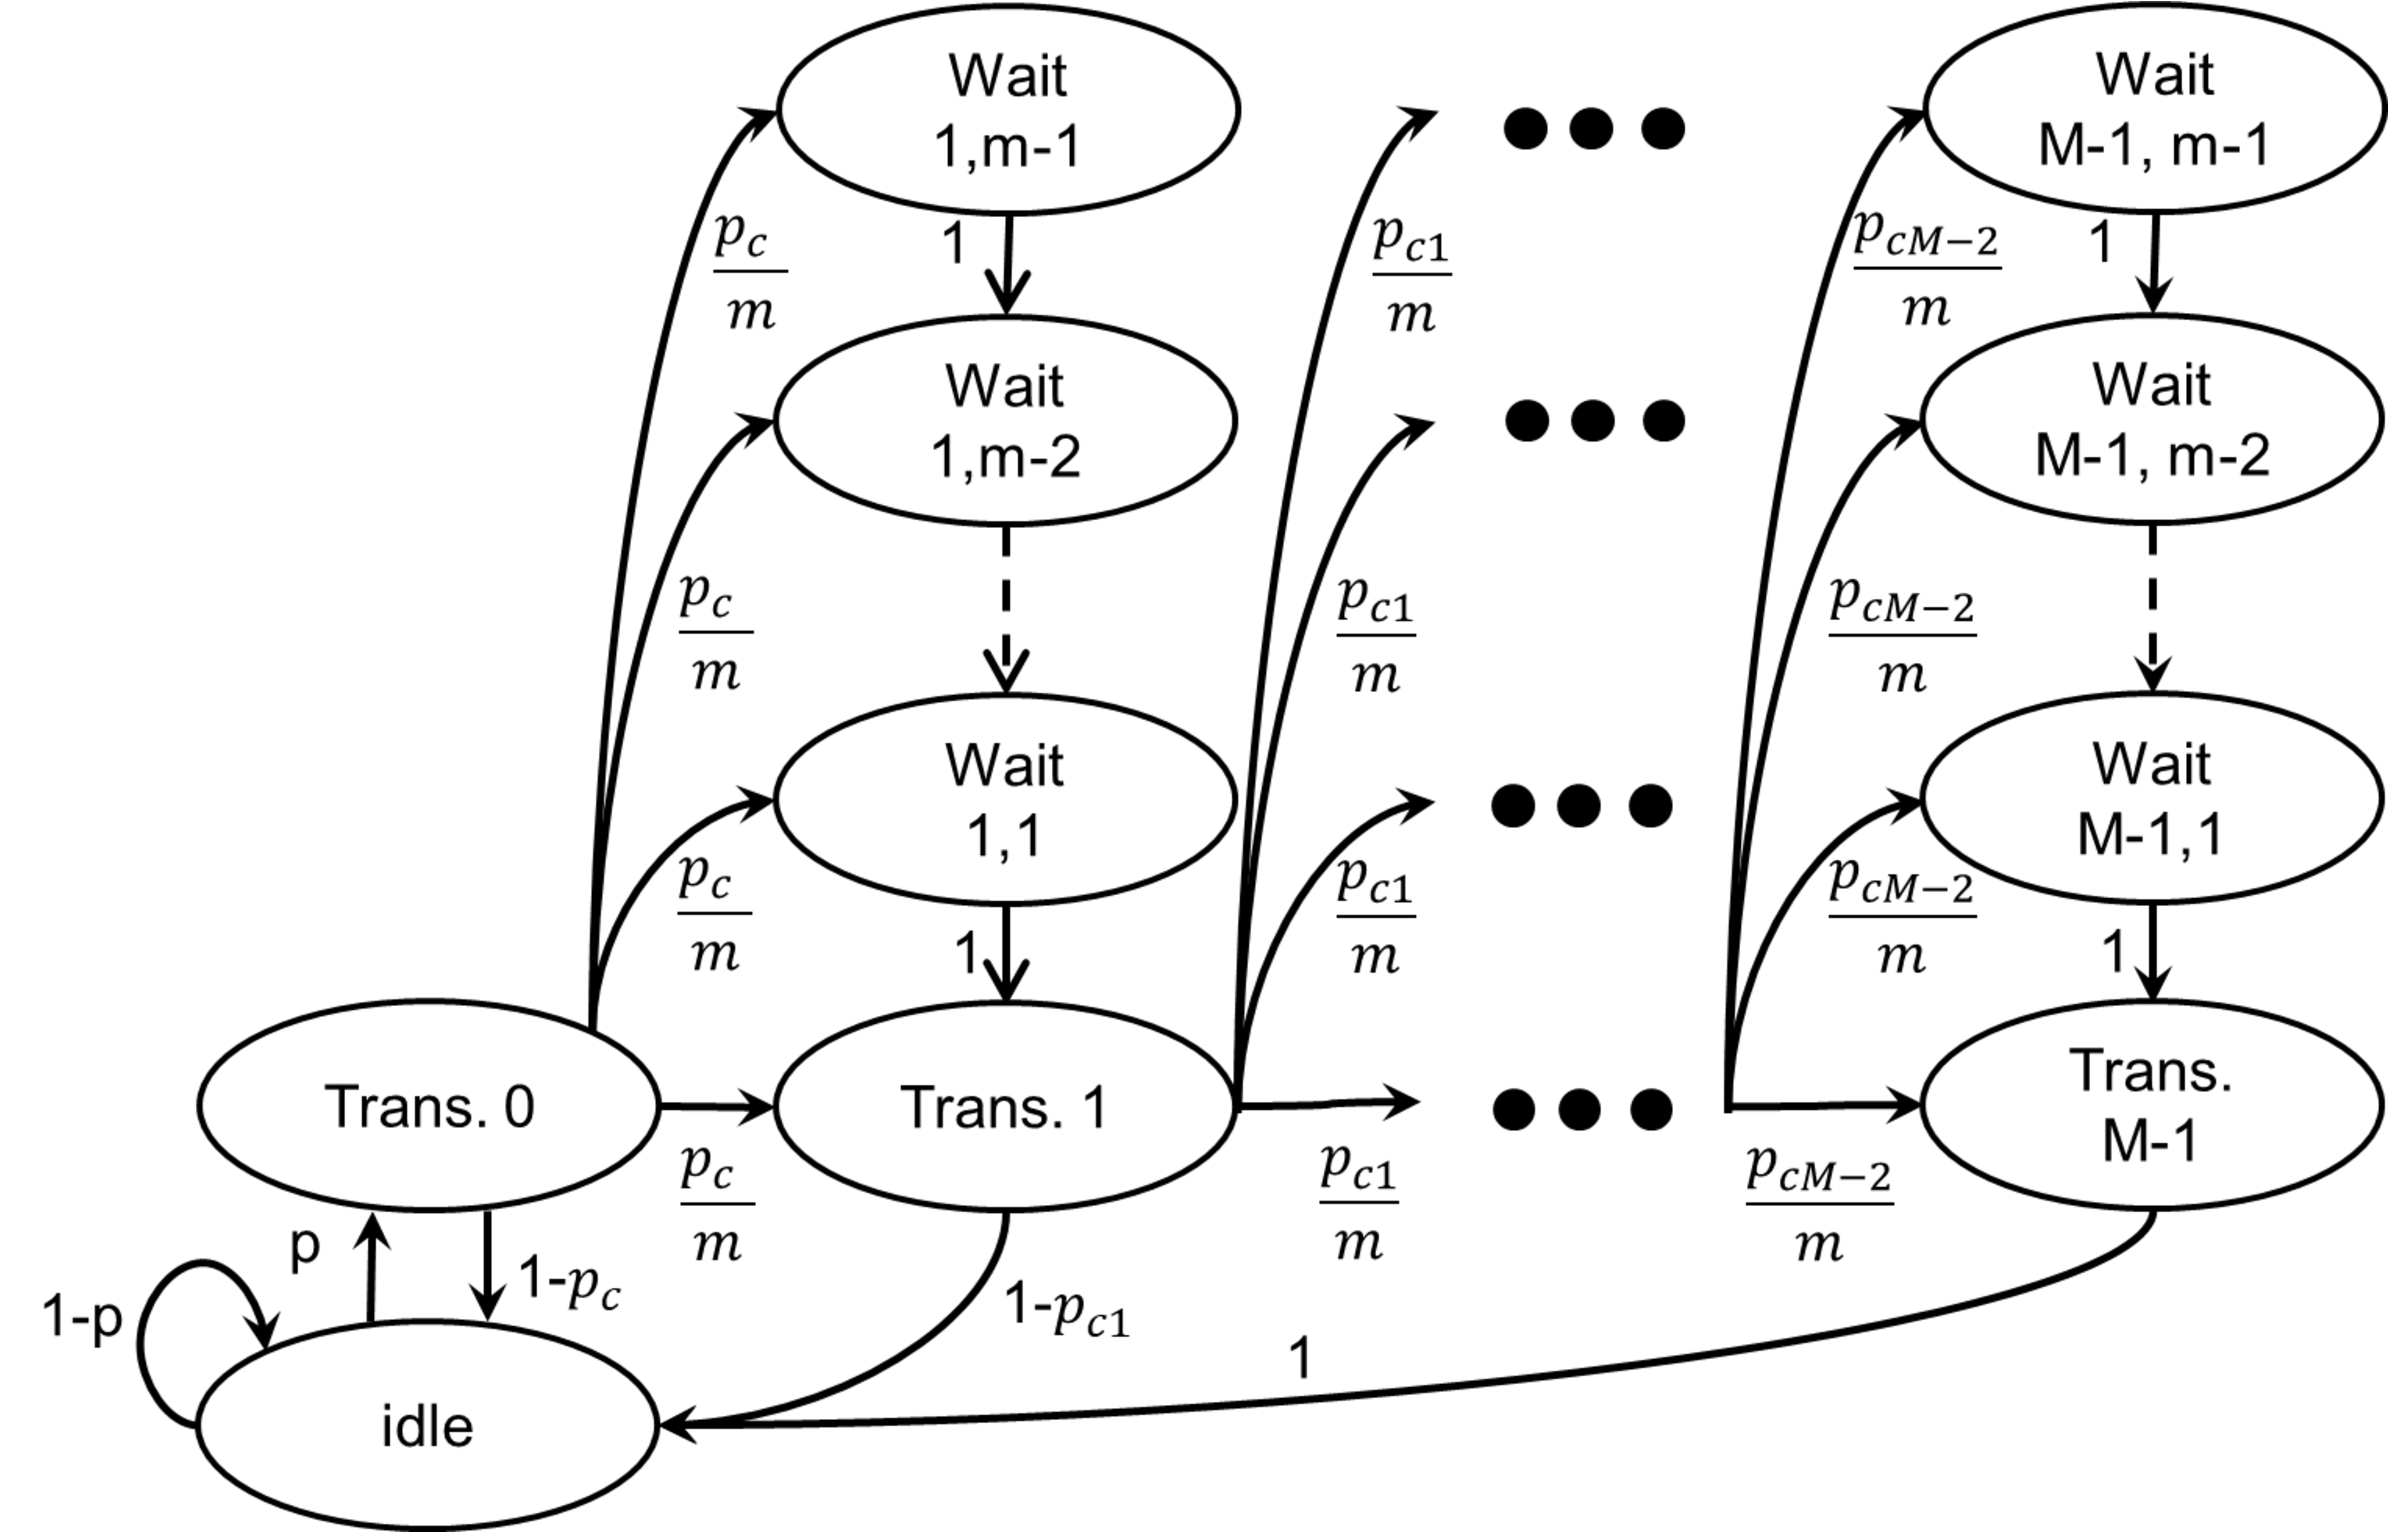
\includegraphics[width=0.70\linewidth]{Markov_model-eps-converted-to.pdf}
	\caption{The Markov model of the behavior of all devices paired to the considered IoT network using the ALOHA protocol. \emph{Note}: $\mathrm{MaxBackOff}$ is written $M$, to have smaller and simpler labels.}
	\label{fig:43:Markov_model}
\end{figure}

A device aims to select a channel with the highest probability of successful transmissions, for which it uses a reinforcement learning approach, again formulated as a MAB problem.
Contrarily to what may appear at first sight,
\emph{the goal is not to minimize the number of retransmissions}, but to maximize the probability of successful transmission, considering both the first transmission of a message and the retransmissions of the same message.
Indeed, the objective of each device is to \emph{maximize its battery life by minimizing its \textbf{total} number of transmissions}.
% , where each channel (also called arms) is viewed as a gambling machine (bandit), and each bandit has a \emph{reward}. Then, at every trial, a device chooses a channel that maximizes the sum of the collected rewards. These \emph{rewards} are the \emph{acknowledgment} (\emph{Ack}) signals received after transmitting packets to the gateway. In this way, a transmission is considered successful when an acknowledgment is received, and a learning approach is employed to select the best channel.
%
We address the problem of channel selection taking into account the described Markov model for the retransmissions of end-devices.
% It motivates our present work for which we consider the retransmissions in the analysis of MAB algorithms.
It motivates our present work for which we consider the number of retransmissions, carried out by each device.
% to address several MAB algorithms.
%

% ----------------------------------------------------------------------
\subsection{Motivations for the proposed approach}
\label{sub:43:motivations}
% ----------------------------------------------------------------------

We consider IoT devices with a constraint on their QoS, imposing the successful delivery of their messages.
When such an IoT device experiments a collision, it goes in a back-off state to retransmit the same packet on the same or another channel.
If all devices remain in the same channel for retransmissions, it is a well-known result that it could result in a sequence of successive collisions with the same packets' devices that previously collided.
%
Thus, it seems interesting to consider in the decision making policy the possibility for a device to retransmit in a different channel.
One of our motivations to develop new MAB algorithms for our problem is this option of using a different communication channel between the first transmission and the next retransmissions.

By considering this possibility, the device will have to learn more, thus, we expect the learning time to be longer, but it could be possible that the final performance gain increases too, in terms of network performance.
We present in Section~\ref{sub:43:numExp} an analysis to check this performance gain, for various heuristics based on the \UCB{} algorithm.
%
Here after, we start by presenting a mathematical derivation that backups this idea.
To do so, we study the collision probabilities considering the Markov process depicted in Figure~\ref{fig:43:Markov_model}, and foresee the impact of using bandit strategies, as well as setting guidelines for the design of heuristic approaches.


\paragraph{Probability of collision at a second transmission slot.}

It is well known \cite{Abramson1970,Roberts75}
that having a collision during an access time can be overcome by a retransmission procedure (this can take several retransmission attempts).
Our goal here is to obtain a mathematical approximation of the collision probability at the second transmission slot $p_{c1}$, as a function of the first collision probability $p_{c}$.
%
We make two approximations $\mathcal{H}_{1}$ and $\mathcal{H}_{2}$ defined as (they are hypotheses on which the rest of this section is built),
\begin{itemize}
	\item $\mathcal{H}_{1}$:
    The probability $p_{c1}$, is composed by the sum of two probabilities: i)
    the probability of colliding consecutively twice, \ie, the devices that collide at a given time slot and collide again when retransmitting their packets,
	and ii) the probability of collision among devices that did not collide in the same previous collision. Moreover, we suppose that the number of devices involved in a collision is small in comparison to the total number of devices.
	This is very realistic as a very small proportion of devices transmit at the same period, due to their low duty cycle.

	\item $\mathcal{H}_{2}$:
	The total number of back-off stages at time $t$ is constant, and it is assumed to be large enough to consider that no device will ever be in the last failure state (this case is the one on the right side in Figure~\ref{fig:43:Markov_model}), after $\mathrm{MaxBackOff}$ successive failed retransmissions
	(otherwise, its battery life can be threatened if it does not have re-fueling capabilities).
\end{itemize}

Considering one device and one channel,
we denote $x_t^i$ the probability that it is transmitting a packet for the $(i+1)$-th time in a given time slot $t$ (with $i\in \{0, \dots, \mathrm{MaxBackOff}-1 \}$),
and we denote $x_t = \sum_{i=0}^{\mathrm{MaxBackOff}-1}x_t^i$ the probability that it transmits a packet (\ie, just the sum on $i$ of $x_t^i$).
We consider $N > 0$ active devices following the same policy.

%{\color{red}Considering one device and a channel,
%we denote $x_t^i$ the packet transmission probability for the $i+1$ time in a given time slot $t$ (with $i\in \llbracket 0, \mathrm{MaxBackOff}-1 \rrbracket$).}
%
%{\color{red}Considering one device and a channel, we denote $x_t^i$ the transmission probability for the $i+1$ time, with $i\in \llbracket 0, \mathrm{MaxBackOff}-1 \rrbracket$, in a given time slot $t$}

We assume to be in the steady state \cite{Norris98}, in our Markov chain model depicted in Figure~\ref{fig:43:Markov_model}, and thus the probabilities no longer depend on the slot number $t$ (\ie, $\forall t, x_t=x$).
Therefore, the probability that this device has a collision at the first transmission is $p_c$, and has the following expression
%
\begin{equation}\label{eq:43:1}
	p_c = 1-\left(1-x\right)^{N-1} \iff x = 1-\left(1-p_c\right)^{\frac{1}{N-1}}.
\end{equation}

Moreover, from \eqref{eq:43:1} we define the probability $p_{cp}(n)$ that involves the collision of $n$ packets sent by each IoT device (for any $1\leq n \leq N-1$), during the first transmission slot, and is defined by $p_{cp}(n) = {N-1 \choose n} \; x^n \left(1-x\right)^{N-1-n}$.
%
As explained above, if an IoT device experiences a collision at the first transmission, it proceeds for the retransmission of its packet after a random back-off interval.
We denote $p_{ca}$ the probability to have a collision with a packet involved in the previous collision.
Under the $\mathcal{H}_{1}$ assumption, the number of packets involved in the same previous collision remains very small in comparison to the total number of devices that may transmit during this time. In other words, this collision probability does not depend on previous retransmissions and is equal to $p_c$.
So, the probability that the same device's packet experiences again a collision at the second time slot is
%
\begin{equation}\label{eq:43:decomppc1}
	p_{c1} = p_{ca}+\left(1-p_{ca} \right)p_c.
\end{equation}


If the device has a collision at the first attempt, we consider $p_{bp}(n)$ the probability that it has a collision with \emph{exactly} $n$ packets (for any $1\leq n \leq N-1$), and that \emph{at least one} of the $n$ devices involved in this first collision chooses the same back-off interval,
%
\begin{equation}
    p_{bp}(n) = {N-1 \choose n} x^n \left(1-x\right)^{N-1-n}\left[1-\left( 1-\frac{1}{m}\right)^n \right].
\end{equation}


Besides, $p_{ca}$ is the conditional probability of collision with a packet sent by a device involved in the previous collision given that the packet experienced collision at its first transmission.
Hence, under hypothesis $\mathcal{H}_{2}$, we can use Bayes theorem and the law of total probability to relate $p_{ca}$ with $p_{bp}(n)$, and the different probabilities that a device experienced a collision during the first slot and has the same back-off interval for its retransmission is,
%{\color{red}Hence, under hypothesis $\mathcal{H}_{2}$,
%the collision probability with the same packets after a retransmission, $p_{ca}$, is given  the sum of collision probabilities with $n$ devices choose the same back-off interval for their retransmissions, }
%
% \begin{equation}\label{eq:43:sumpca}
	$p_{ca} = \frac{1}{p_c}\sum_{n=1}^{N-1} p_{bp}(n)$.
% \end{equation}
%
% \begin{figure}[htp!]  % [htbp]
% 	\centering
% 	% 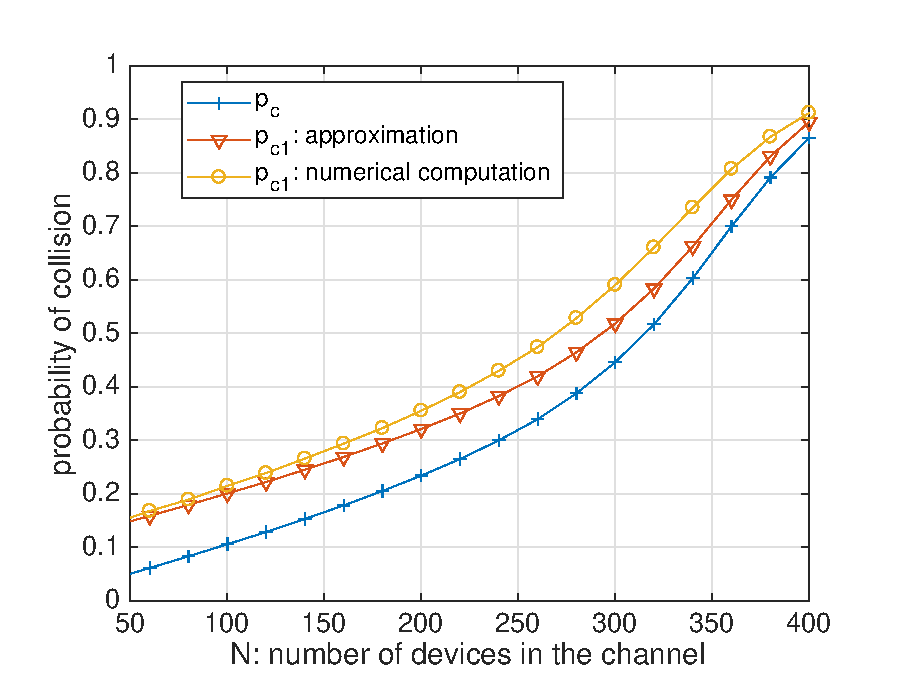
\includegraphics[width=1.00\linewidth]{Approximation_m10.eps}
% 	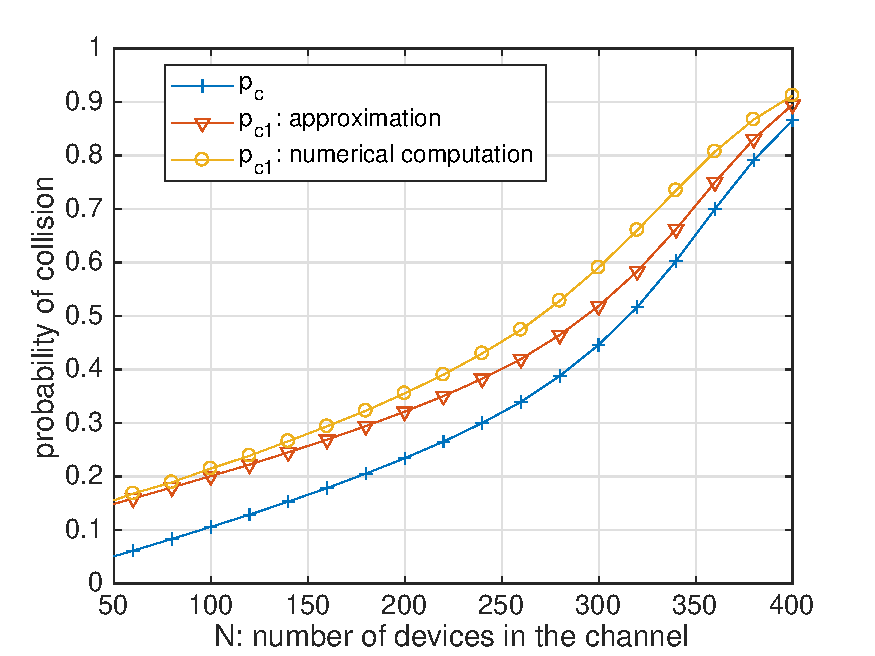
\includegraphics[width=1.00\linewidth]{Approximation_m10-eps-converted-to.pdf}
% 	\caption{Our proposed approximation for the probability of collision at the second transmission. It is more precise for smaller values of $N$.}
% 	\label{fig:43:Approximation_m10}
% \end{figure}
%
Therefore, the expression of $p_{ca}$ is
%
\begin{align}\label{eq:43:sumpc2}
	& \frac{1}{p_c} \sum_{n=1}^{N-1}{N-1 \choose n} x^n \left(1-x\right)^{N-1-n}\left[1-\left( 1-\frac{1}{m}\right)^n \right]\nonumber \\
	& = 1- \frac{1}{p_c}\sum_{n=1}^{N-1}{N-1 \choose n} x^n \left(1-x\right)^{N-1-n}\left( 1-\frac{1}{m}\right)^n.
\end{align}

Once again under $\mathcal{H}_{1}$, assuming that the number of devices involved in the first collision is small compared to $N-1$, the first $N_0 \ll N-1$ terms of the sum in \eqref{eq:43:sumpc2} are predominant. We derive $p_{ca} \simeq  1- \frac{1}{p_c}\sum_{n=1}^{N_0}{N-1 \choose n} x^n\left(1-x\right)^{N-1-n} \left( 1-\frac{1}{m}\right)^n$.
%
Moreover, for these terms, $n$ is small compared to $N-1$, and so $N-1-n$ can be approximated to $N-1$. Thus it gives,
%
\begin{equation}\label{eq:43:sumpca3}
	p_{ca} \simeq  1- \frac{\left(1-x\right)^{N-1}}{p_c}\sum_{n=1}^{N_0}{N-1 \choose n} x^n \left( 1-\frac{1}{m}\right)^n.
\end{equation}

Assuming $\mathcal{H}_{1}$ amounts to consider that $x\ll 1$. As a consequence, the sum in equation \eqref{eq:43:sumpca3} can be supplemented by negligible terms,
%
\begin{equation}\label{eq:43:sumpca4}
	p_{ca} \simeq  1 - \frac{\left(1-x\right)^{N-1}}{p_c}\sum_{n=1}^{N-1}{N-1 \choose n} x^n \left( 1-\frac{1}{m}\right)^n.
\end{equation}

The binomial theorem expands the sum in \eqref{eq:43:sumpca4}, so we can rewrite the expression of $p_{ca}$
%
\begin{equation}\label{eq:43:pca}
	p_{ca} \simeq 1 - \left(\frac{1}{p_c}-1\right)\left[ 1+\left(1-\left(1-p_c\right)^{\frac{1}{N-1}}\right)\left(1-\frac{1}{m}\right)\right]^{N-1}.
\end{equation}

Finally, our approximation of $p_{c1}$ can be obtained by inserting \eqref{eq:43:pca} in \eqref{eq:43:decomppc1}.
%
\begin{align}\label{eq:43:final_expression_pc1}
	p_{c1} &= p_{ca}+\left(1-p_{ca}\right)p_c = (1 - p_c) p_{ca} + p_c \nonumber \\
	&\simeq \left(1 - p_c\right) (1 - \left(\frac{1}{p_c}-1\right)\left[ 1+\left(1-\left(1-p_c\right)^{\frac{1}{N-1}}\right)\left(1-\frac{1}{m}\right)\right]^{N-1} + p_c.
\end{align}


% --- --- --- --- --- --- --- --- --- ---
\paragraph{Behavior analysis of $p_{c}$ and $p_{c1}$}\label{sub:43:numericalValidationPC1PC}

In order to assess the proposed approximation, we suppose a unique channel where all the devices follow the same contention Markov process.
We simulate an ALOHA protocol with a maximum number of retransmissions $\mathrm{MaxBackOff}=10$, a maximum back-off interval $m=10$, and a transmission probability $p=10^{-3}$.
%
In Figure~\ref{fig:43:Approximation_m10}, we show the collision probabilities for different number of devices $N$ (from $N=50$ to $N=400$), for both $p_{c}$ and $p_{c1}$.
%
We can verify that our approximation is very precise for lower values $p_{c1} \leq 30 \%$ (\ie, \textcolor{red}{red} and \textcolor{gold}{orange} curves are quite close).
Moreover, a significant gap between $p_{c1}$ and $p_c$,
of up-to $10\%$, can be observed,
which suggests us to resort to MAB algorithms for the channel selection for both the first transmission and next retransmissions.

\begin{figure}[htp!]  % [htbp]
	\centering
	% 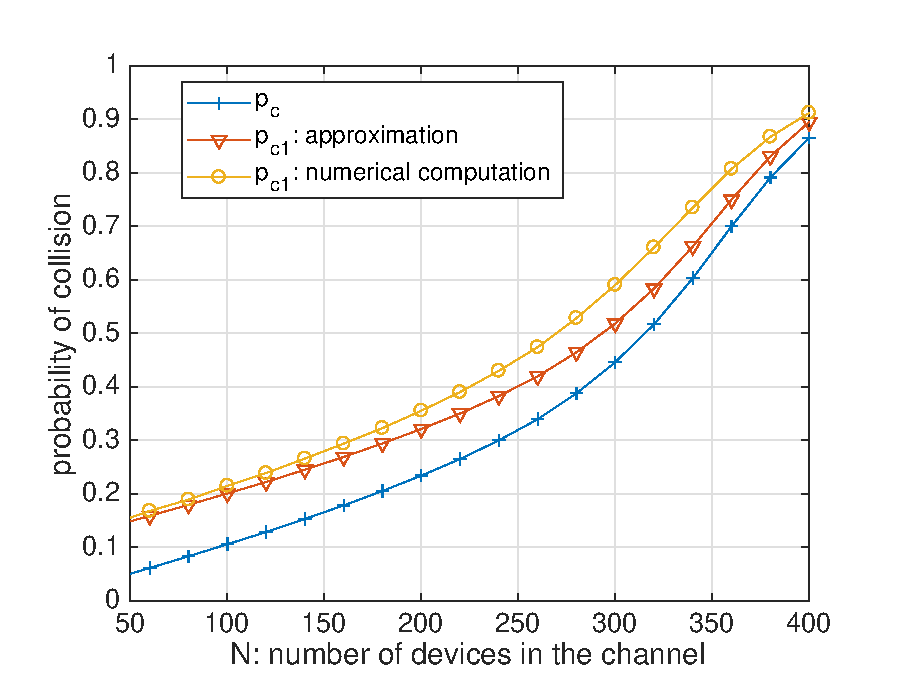
\includegraphics[width=0.65\linewidth]{Approximation_m10.eps}
	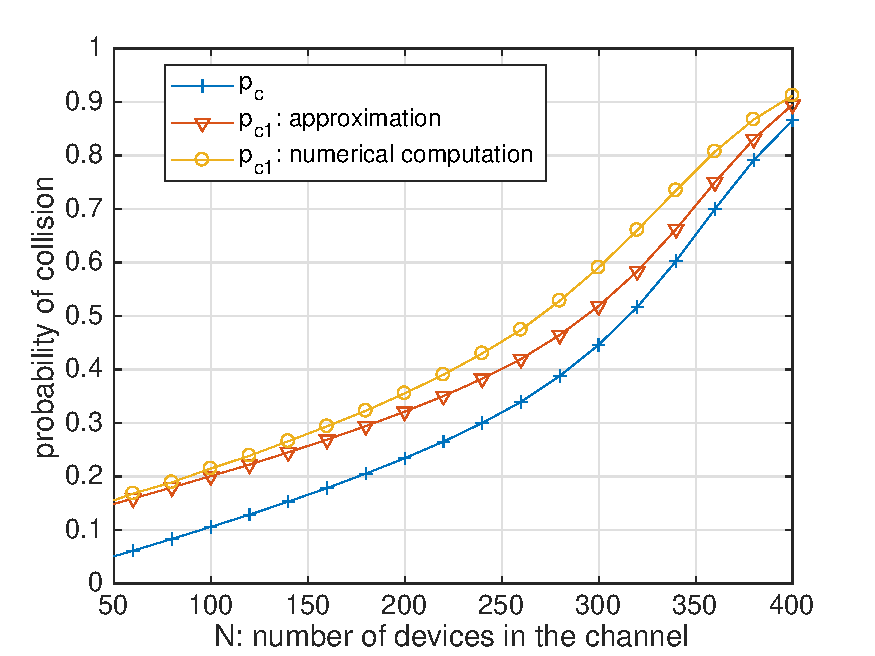
\includegraphics[width=0.60\linewidth]{Approximation_m10-eps-converted-to.pdf}
	\caption[Our approximation for the probability of collision at the second transmission.]{\textcolor{red}{Our approximation (in red)} of \textcolor{gold}{$p_{c1}$ (in orange)}, probability of collision at the second transmission, is more precise for smaller $N$. We also include \textcolor{blue}{$p_{c}$ (in blue)}.}
	\label{fig:43:Approximation_m10}
\end{figure}


\paragraph{Learning is useful for non-congested networks.}

It is worth to highlight that, if we write \eqref{eq:43:decomppc1} as $p_{c1} = p_c + p_{ca} \left(1-p_c\right)$,
then it is obvious that $p_{c1}$ is always larger than $p_c$ (as $p_{ca} \left(1-p_c\right) > 0$).
But for large values of $p_c$, $p_{ca}\left(1-p_c\right) \simeq 0$ so the gap gets small,
and for small values of $p_c$ the gap is significant.
Moreover, we can verify (\eg, numerically or by differentiating)
that the gap decreases when $p_c$ increases (for fixed $N$ and $m$).
This backups mathematically the observation we made from Figure~\ref{fig:43:Approximation_m10}:
the smaller the $p_c$, the larger is the gap between $p_c$ and $p_{c1}$.
%
We interpret this fact in two different situations:
\begin{itemize}
	\item
	On the one hand, in a congested network, when devices suffer from a large probability of collision on their first transmission (\ie, $p_c$ is not so small), then $p_{c1}\simeq p_c$ and so devices cannot really hope to reduce their collision probabilities even if the use a different channel for retransmission.
	\item
	On the other hand, if $p_c$ is small enough, \ie, in a network not yet too congested, then our derivation shows that $p_{c1} > p_c$, meaning that the possible gain of retransmitting in a different channel that the one used for the first transmission can be large, in terms of collision probability (\eg, up-to $10\%$ in this experimental setting).
	In other words, when learning can be useful (small $p_c$), learning to retransmit in a different channel can have a large impact on the global collision rate,
	thus justifying our approach.
\end{itemize}

% %-----------------------------------------------------------------
% \subsection{The \UCB{} algorithm as a building block for different heuristics}
% \label{sub:43:MABalgo}
% % ----------------------------------------------------------------------

% Before presenting our proposed heuristics, we remind here the \UCB{} bandit algorithm \cite{Auer02}.
% We include it again to facilitate the understanding of the heuristics, which use \UCB{} as a building block.


% % % --- --- --- --- --- --- --- --- --- ---
% \paragraph{The \UCB{} algorithm.}\label{sub:43:algoUCB}

% More formally, for one device, let $N_k(t)$ be the number of times the channel $k$ (for $k\in \llbracket 1, K \rrbracket$) was selected up-to time $t-1$, for $t\geq 0$
% for any $t\in\mathbb{N}$,
% \begin{equation}\label{eq:43:Nkt}
% 	N_k(t) = \sum_{\tau=0}^{t-1} \mathbbm{1}(A(\tau) = k),
% \end{equation}
% The empirical mean estimator $\widehat{\mu_k}(t)$ of channel $k$ is defined as the mean reward obtained up-to time $t-1$,
% \begin{equation}\label{eq:43:mukt}
% 	\widehat{\mu_k}(t) = \frac{1}{N_k(t)} \sum_{\tau=0}^{t-1} r_k(\tau) \mathbbm{1}(A(\tau) = k).
% \end{equation}
% where $r_{k}(t)$ is the reward obtained after transmission in channel $k$ at time $t$ ($1$ for a successful transmission, and $0$ otherwise)
% %
% A \emph{confidence} term $B_k(t)$ is given by \cite{Auer02},
% \begin{equation}\label{eq:43:Bkt}
% 	B_k(t) = \sqrt{\alpha \log(t) / N_k(t)},
% \end{equation}
% where $\alpha$ refers to an exploration coefficient,
% % \footnote{~In fact, the larger this coefficient is, the longer the exploration, while the \UCB{} algorithm is proven to be order optimal for $\alpha>0.5$ \cite{Bubeck12}, and has reported a good performance for lower values of $\alpha>0$.},
% that we chose equal to $1/2$, as suggested in \cite{Audibert07} and as done in previous works \cite{Bonnefoi18,Bonnefoi17}.
% Then, an upper confidence bound in each channel $k$ is defined as
% \begin{equation}\label{eq:43:ucb}
% 	U_k(t) = \widehat{\mu_k}(t) + B_k(t).
% \end{equation}
% Finally, the transmission channel at time step $t$
% is the one maximizing this \UCB{} index $U_k(t)$,
% as it is the one expected to be the best one at the current time step $t$,
% \begin{equation}\label{eq:43:maxucb}
% 	A(t) \sim \cU(\argmax_k U_k(t)).
% \end{equation}

% The \UCB{} algorithm is implemented independently by each device, and we present it in Algorithm~\ref{algo:43:UCB}.
% Note that a device using this first approach is only able to select a channel for the first and all the corresponding retransmissions of a packet.

% % \begin{small} % XXX remove if needed
% \begin{figure}[h!]
% 	\centering
%     \begin{framed}
% 	\begin{algorithm}[H]
		% \begin{small} % XXX remove if needed
% 		\For(){$t = 1, \dots, T$}{
% 			Compute $\forall k, U_k(t) = \widehat{\mu_k}(t) + \sqrt{\alpha \log(t) / N_k(t)}$\;
% 			Transmit in channel $A(t) \sim \cU(\argmax_k U_k(t))$\;
% 			Reward $r_{A(t)}(t) = 1$, if \emph{Ack} is received, else $0$\;
% 		}
% 		\caption{The \UCB{} algorithm for channel selection (base building block).}
% 		\label{algo:43:UCB}
		% \end{small} % XXX remove if needed
% 	\end{algorithm}
% 	\end{framed}
% \end{figure}
% % \end{small} % XXX remove if needed

% ----------------------------------------------------------------------
\subsection{The first heuristic: \UCB{} unaware of retransmissions}
\label{sub:43:UCBnaive}
% ----------------------------------------------------------------------

% \paragraph{First stage \UCB.}\label{sub:43:firstStageUCB}

This first heuristic we propose is unaware of retransmission: the same channel is used for retransmissions.
The \UCB{} algorithm is implemented independently by each device, we denote it ``first-stage'' \UCB, and we present it in Algorithm~\ref{algo:43:UCB}.
It is the same algorithm as the Algorithm~\ref{algo:2:indexPolicy} in Section~\ref{sub:2:IndexPolicies} (using the same \UCB{} indexes as we defined them in equation \eqref{eq:2:UCB_index}),
but we write it again to make clear the difference with first transmission and retransmission of messages.
%
Note that a device using this first approach is only able to select a channel for the first transmission (using \UCB, line 3-5), and then it uses the same channel for all the corresponding retransmissions of a packet (if retransmissions happen, line 7-8).


% \begin{small} % XXX remove if needed
\begin{figure}[h!]
	\centering
    \begin{framed}
	\begin{algorithm}[H]
		% \begin{small} % XXX remove if needed
		\For(){$t = 1, \dots, T$}{
			\uIf{First packet transmission}{
				Compute $\forall k, U_k(t) = \widehat{\mu_k}(t) + \sqrt{\alpha \log(t) / N_k(t)}$\;
				Transmit in channel $A(t) \sim \cU(\argmax_k U_k(t))$\;
				Reward $r(t) = 1$, if \emph{Ack} is received, else $0$\;
			}
			\uElse(\tcp*[f]{Retransmit in same channel}){
				j $\leftarrow$ last channel selected by first-stage \UCB\;
				Transmit in channel $A(t) = j$\;
			}
		}
		\caption[First-stage \UCB{} and retransmission in same channel.]{First-stage \UCB{} and retransmission in same channel (``\textcolor{blue}{Only \UCB{}}'').}
		\label{algo:43:UCB}
		% \end{small} % XXX remove if needed
	\end{algorithm}
	\end{framed}
\end{figure}
% \end{small} % XXX remove if needed


More formally, for one device, let $N_k(t)$ be the number of times the channel $k$ (for $k\in [K]$) was selected up-to time $t-1$, for $t\geq1$
for any $t\in\mathbb{N}$,
$N_k(t) = \sum_{\tau=1}^{t-1} \mathbbm{1}(A(\tau) = k)$.
The empirical mean estimator $\widehat{\mu_k}(t)$ of channel $k$ is defined as $\widehat{\mu_k}(t) = \frac{1}{N_k(t)} \sum_{\tau=1}^{t-1} r(\tau) \mathbbm{1}(A(\tau) = k)$,
where $r(t)=Y_{k,t}$ is the reward obtained after transmission in channel $k$ at time $t$.
The upper confidence bound in each channel $k$ is defined as
$U_k(t) = \widehat{\mu_k}(t) + \sqrt{\alpha \log(t) / N_k(t)}$.
Finally, the transmission channel at time step $t$
is $A(t) \sim \cU(\argmax_k U_k(t))$.
% the one maximizing this \UCB{} index $U_k(t)$,
% as it is the one expected to be the best one at the current time step $t$,

\begin{leftbar}[warningbar]  % XXX leftbar warningbar, comment if needed
	% \begin{small}  % XXX WARNING
		\textbf{\textcolor{red}{Small warning about notations: local (device) time vs global (gateway) time}.}
		%
		In the algorithms presented in this chapter, the time step $t$ does not refer to the \emph{global} time step (as seen from the gateway), but rather the current number of uplink transmissions (or retransmissions) that was carried out by the device.
		Each device wakes up whenever it has to send some data, following its own emission process (we restrict to a Bernoulli process of small probability, \eg, $p=10^{-3}$), and whenever it wakes up, it sends its packet, and will send again for at most $\mathrm{MaxBackOff}$ times (\eg, $\mathrm{MaxBackOff}=10$) until it receives an \Ack.
		%
		In other words, the time steps $t$ in the following algorithms denote the number of uplink packets sent by the device, and these uplink transmissions or retransmissions can happen at different (global or real-world) times.
		The local index $t$ is independent on the global time (\ie, the time of the gateway), and IoT device does not need to care about this difference.
		From the device point-of-view, the learning occurs at successive times (whenever the device wakes up), regardless of the global time.
	% \end{small}  % XXX WARNING
\end{leftbar}  % XXX leftbar warningbar, comment if needed


% ----------------------------------------------------------------------
\subsection{Heuristics to (try to) learn how to retransmit efficiently}
\label{sub:43:heuristics}
% ----------------------------------------------------------------------

A device that implements the UCB algorithm is led to focus its transmissions and retransmissions in the channel which is currently identified as the best.
As explained above in Section~\ref{sub:43:motivations}, focusing in one channel could increase the collision probability in retransmissions.
We describe here the proposed heuristics for the channel selection in a retransmission. It is carried out taking into account that a device can incorporate a different channel selection strategy while being in a back-off state.
Hence, a natural question is to evaluate whether using this additional contextual information can improve the performance of a learning policy.

For that end, all of our heuristics comprise two stages:
the first stage is a \UCB{} algorithm employed for the first attempt to transmit,
and the second stage is another algorithm used for channel selections for the next retransmissions.
%
We present below four heuristics for this second stage.
Their short names (with their colors) are used in the legend on Figures~\ref{fig:43:mainExperiment1}, \ref{fig:43:mainExperiment2}), and are given in ``quotes'' in the corresponding paragraphs.


% --- --- --- --- --- --- --- --- --- ---
\paragraph{Uniform random retransmission ``(\textcolor{cyan}{Random}'').}\label{sub:43:UCBthenRandom}
%
In this first proposal, the device uses a random channel selection, following a uniform distribution (on $[K]$).
It is described below in Algorithm~\ref{algo:43:UCBthenRandom}.
More precisely, the first-stage \UCB{} use rewards built from the acknowledgments that the device received or not for its first-stage transmission, but do not use any feedback about any of the retransmissions of any message.

% \vspace*{-3pt}
\begin{figure}[h!]
	\centering
    \begin{framed}
	\begin{algorithm}[H]
	% \begin{small} % XXX remove if needed
	\For(){$t = 1, \dots, T$}{
			\uIf{First packet transmission}{
				Use first-stage \UCB{} as in Algorithm~\ref{algo:43:UCB}\;
			}
			\uElse(\tcp*[f]{Random retransmission}){
				Transmit in channel $A(t) \sim \mathcal{U}(1,\ldots,K)$\;
			}
		}
		\caption[Heuristic: uniform random retransmission.]{Heuristic: uniform random retransmission ``(\textcolor{cyan}{Random}'').}    % A naive
		\label{algo:43:UCBthenRandom}
	% \end{small} % XXX remove if needed
	\end{algorithm}
	\end{framed}
\end{figure}


% --- --- --- --- --- --- --- --- --- ---
\paragraph{\UCB{} for retransmission (``\textcolor{purple}{\UCB{}}'').}\label{sub:43:TwoUCB}
%
Instead of applying a random channel selection for retransmission,
another heuristic is to use a second \UCB{} algorithm in the second stage.
In other words, we expect that this algorithm is able to learn the best channel to retransmit a packet.
It is described in Algorithm~\ref{algo:43:TwoUCB}, and it is still a practical approach, since the storage requirements and time complexity remains linear w.r.t. the number of channels $K$ (\ie, $\mathcal{O}(K)$).
%
Note that, we use the subscript $({}^r)$ to denote the variables
$\widehat{\mu}^r(t)$, $B^r_k(t)$ and $U^r_k(t)$,
related to the \UCB{} algorithm employed for the retransmission.

% \vspace*{-3pt}
% \begin{small} % XXX remove if needed
\begin{figure}[h!]
	\centering
    \begin{framed}
	\begin{algorithm}[H]
		% \begin{small} % XXX remove if needed
		\For(){$t = 1, \dots, T$}{
			\uIf{First packet transmission}{
				Use first-stage \UCB{} as in Algorithm~\ref{algo:43:UCB}\;
			}
			\uElse(\tcp*[f]{Packet retransmission with the other $\mathrm{UCB}^r$}){
				Compute $\forall k, U^r_k(t) = \widehat{\mu_k}^r(t) + \sqrt{\alpha \log(t) / N_k^r(t)}$\;
				Transmit in channel $C^r(t) \sim \cU(\argmax_k U^r_k(t))$\;
				Reward $r^r(t) = 1$, if \emph{Ack} is received, else $0$\;
			}
		}
		\caption[Heuristic: \UCB{} for retransmission.]{Heuristic: \UCB{} for retransmission (``\textcolor{purple}{\UCB{}}'').}    % A naive
		\label{algo:43:TwoUCB}
		% \end{small} % XXX remove if needed
	\end{algorithm}
	\end{framed}
\end{figure}
% \end{small} % XXX remove if needed


% --- --- --- --- --- --- --- --- --- ---
\paragraph{$K$ different {\UCB}s for retransmission (``\textcolor{green}{$K$ \UCB}'')}\label{sub:43:UCBthenKp1}
%
Another heuristic is to not use the same algorithm no matter where the collision occurred, but to use $K$ different second-stage \UCB{} algorithms.
It means that after a failed first transmission in channel $j$, the device relies on the $j$-th algorithm to decide its retransmission.
The corresponding algorithm is depicted in Algorithm~\ref{algo:43:UCBthenKp1}.
Each of these algorithms are denoted using the subscript $({}^{j})$, for $j\in[K]$.

% \vspace*{-3pt}
% \begin{small} % XXX remove if needed
\begin{figure}[h!]
	\centering
\begin{framed}
	\begin{algorithm}[H]
		% \begin{small} % XXX remove if needed
		% \KwData{$\forall k,j\in[\![1;K]\!]$, $N_k^j(t)$, $\widehat{\mu_k}^j(t)$, $B_k^j(t)$ and $U_k^j(t)$}
		\For(\tcp*[f]{At every time step})
		{$t = 1, \dots, T$}{
			\uIf{First packet transmission}{
				Use first-stage \UCB{} as in Algorithm~\ref{algo:43:UCB}\;
			}
			\uElse(\tcp*[f]{Packet retransmission with one of the $K$ $\mathrm{UCB}^j$}){ % Retr. after trying channel $j$
				j $\leftarrow$ last channel selected by first-stage \UCB\;
				Compute $\forall k, U_k^j(t) = \widehat{\mu_k}^j(t) + \sqrt{\alpha \log(t) / N_k^j(t)}$\;
				Transmit in channel $A^j(t) \sim \cU(\argmax_k U^j_k(t))$\;
				Reward $r^j_{A^j(t)}(t) = 1$ if \emph{Ack} is received, else $0$\;
			}
		}
		\caption[Heuristic: $K$ different {\UCB}s for retransmission.]{Heuristic: $K$ different {\UCB}s for retransmission (``\textcolor{green}{$K$ \UCB}'').}
		\label{algo:43:UCBthenKp1}
		% \end{small} % XXX remove if needed
	\end{algorithm}
	\end{framed}
\end{figure}
% \end{small} % XXX remove if needed

Although, this approach increases the complexity and storage requirements (now, of order $\mathcal{O}(K^2)$).
For our LPWA networks of interest, such as LoRaWAN, the cost of its implementation is still affordable, since a small number of channels is used.
For instance, for $K=4$ channels,
the memory to store $K+1=5$ algorithms is of the order of the requirements to store one.

Note that for other networks this heuristic could not be practical.
The storage requirements and time complexity is now quadratic in $K$, and as such we no longer consider this heuristic to be a practical proposal in some LPWA networks, as for instance Sigfox networks consist in a large number of very narrow-band channels (\eg, $K=128$).
But for LoRaWAN networks with $K=4$, storing $K+1=5$ algorithms does not cost much more than storing $2$.


% --- --- --- --- --- --- --- --- --- ---
\paragraph{Delayed \UCB{} for retransmission (``\textcolor{red}{Delayed \UCB}'').}\label{sub:43:UCBwithDelay}
%
This last heuristic is a composite of
the random retransmission (Algorithm~\ref{algo:43:UCBthenRandom})
and the \UCB{} retransmission (Algorithm~\ref{algo:43:TwoUCB}) approaches.
Instead of starting the second stage \UCB{} directly from the first retransmission, we introduce a fixed delay $\Delta\in\mathbb{N}$, $\Delta \geq 1$,
and start to rely on the second stage \UCB{} after $\Delta$ transmissions.
The selection for the first steps is handled with the random retransmission.

The idea behind this delay is to allow the first stage \UCB{} to start learning the best channel, before starting the second stage \UCB{} (see details in Algorithm~\ref{algo:43:UCBwithDelay}).
The number of transmissions to wait before applying the second algorithm is denoted by $\Delta$, it has to be fixed before-hand\footnote{~Choosing the value of $\Delta$ could be done by extensive benchmarks but such approach goes against the reinforcement learning idea: an heuristic should work against any problem, without the need to simulate the problem before-hand to find a good value of some internal parameter. As such, we only consider a delay of $\Delta=100$ in our experiments, and we did not try to optimize it.}.
%
Note that, we use the subscript $({}^d)$ to denote the variables
related to the delayed second-stage \UCB{} algorithm.

% \vspace*{-3pt}
% \begin{small} % XXX remove if needed
\begin{figure}[h!]
	\centering
	\begin{framed}
	\begin{algorithm}[H]
		% \begin{small} % XXX remove if needed
		\For(\tcp*[f]{At every time step})
		{$t = 1, \dots, T$}{
			\uIf{First packet transmission}{
				Use first-stage \UCB{} as in Algorithm~\ref{algo:43:UCB}\;
			}
			\uElseIf(\tcp*[f]{Random retransmission}){$t \leq \Delta$}{
				Transmit randomly in a channel $A(t) \sim \mathcal{U}(1,\ldots,K)$.
			}
			\uElse(\tcp*[f]{Packet retransmission with delayed $\mathrm{UCB}^d$}){
				Compute $\forall k, U^d_k(t) = \widehat{\mu_k}^d(t) + \sqrt{\alpha \log(t) / N_k^d(t)}$\;
				Transmit in channel $A^d(t) \sim \cU(\argmax_k U^d_k(t))$\;
				Reward $r^d_{A^d(t)}(t) = 1$ if \emph{Ack} is received, else $0$\;
			}
		}
		\caption[Heuristic: delayed \UCB{} for retransmission.]{Heuristic: delayed \UCB{} for retransmission (``\textcolor{red}{Delayed \UCB}'').}
		\label{algo:43:UCBwithDelay}
		% \end{small} % XXX remove if needed
	\end{algorithm}
	\end{framed}
\end{figure}
% \end{small} % XXX remove if needed


\paragraph{Other ideas that we did not explore.}
%
Instead of considering a first-stage \UCB{} followed by a random channel retransmission, we could have considered a random first-stage channel retransmission followed by a second-stage \UCB.
This was not considered in our study \cite{Bonnefoi2019WCNC}, and we preferred to not add it to the experiments presented below, for three reasons: to avoid clutter in the plots, to win some time as these experiments had to run for quite a long time, but mainly because the first-stage channel selection is most important one as we illustrate by the large difference in terms of performance between the uniform channel selection and the ``Only UCB'' heuristic, below in Figures~\ref{fig:43:mainExperiment1} and \ref{fig:43:mainExperiment2}.


\paragraph{Using another bandit policy?}
%
% Similarly, Philippe Mary asked me at the MoTION workshop where I presented \cite{Bonnefoi2019WCNC}, why didn't we rather used Bayes-UCB instead of \UCB{} (from \cite{Kaufmann12BUCB}), as it is known to empirically outperform \UCB{} (as illustrated for instance in \cite{darak2016bayesian,kumar2016two}).
We could have chose any bandit algorithm for the ``first stage'' component used in this Section, and for simplicity and clarity we focused on a simple but efficient one (\UCB).
We believe that the same empirical results, but more importantly, the same conclusions, could be given if we used Bayes-UCB or other bandit algorithm for the base building block in the different heuristics proposed in this section.
% ~\ref{sub:43:heuristics}.
Our goal here was not to optimize on the bandit policy (as we presented in Section~\ref{sec:3:reviewSPAlgorithms} some numerical simulations doing precisely this), but rather to compare the different heuristics, for a fixed bandit policy (for which we preferred to use \UCB{} for simplicity).


% ----------------------------------------------------------------------
\subsection{Numerical results}
\label{sub:43:numExp}
% ----------------------------------------------------------------------

We simulate our network considering $N$ devices following the contention Markov process described in Section~\ref{sub:43:model}, and a LoRaWAN standard with $K=4$ channels, as in Section~\ref{sec:4:firstModel}.
Each device is set to transmit with a fixed probability $p=10^{-3}$, \ie, a packet about every $20$ minutes for time slots of \SI{1}{\second}.
% $1\;\mathrm{s}$.
%
For the evaluation of the proposed heuristics, a total number of $T=20 \times 10^4$ time slots is considered, and the results are averaged over $1000$ independent random simulations.
%In this way, it allows us to evaluate the learning rate, as well as the convergence of each learning approach.

In a first scenario, we consider a total number of $N=1000$ IoT devices, with a non-uniform repartition of static devices given by $10\%,30\%,30\%,30\%$ for the four channels.
In other words, the channels are occupied\footnote{~Note that we consider higher occupancy rates that the ones considered previously in Section~\ref{sec:4:gnuradio}, because the goal of this experimental section is to evaluate our approach that uses learning to optimize the way each device retransmits its packets. We need to have a large enough probability $p_c$ of retransmission if we want to see a difference between the different learning heuristics, which is why we consider a network more densely occupied than the one considered in Section~\ref{sec:4:gnuradio}.}
respectively $10\%$, $30\%$, $30\%$, and $30\%$ of time, and the contention Markov process considered is given by $\mathrm{MaxBackOff} = 5$, and $m=5$.
In Figure~\ref{fig:43:mainExperiment1}, we show the successful transmission rate versus the number of slots, for all the proposed heuristics.

A first result is that all the heuristics clearly outperform the non-learning approach that simply uses random channel selection for both transmissions and retransmissions (\ie, the ``no \UCB{}'' curve in black), which is (still) the current state-of-the-art in IoT networks.
The improvement of the heuristics over the non-learning approach is clear, and for every heuristic that uses a kind of learning mechanism it can be observed that the successful transmission rate increases rapidly (or equivalently the PLR decreases).
Moreover, all of these approaches show a fast convergence making them suitable for the targeted application.
It is also worth mentioning that the employment of the same \UCB{} algorithm for retransmissions, denoted here as ``Only \UCB{}'', achieves a better performance, while a ``Random'' retransmission features a slight degradation. This result can be explained as follows: the loss of performance related to the separation of information for several algorithms is greater than the gain obtained by considering the first transmissions and retransmissions separately.

\begin{figure}[h!]  % [htbp]
	\centering
	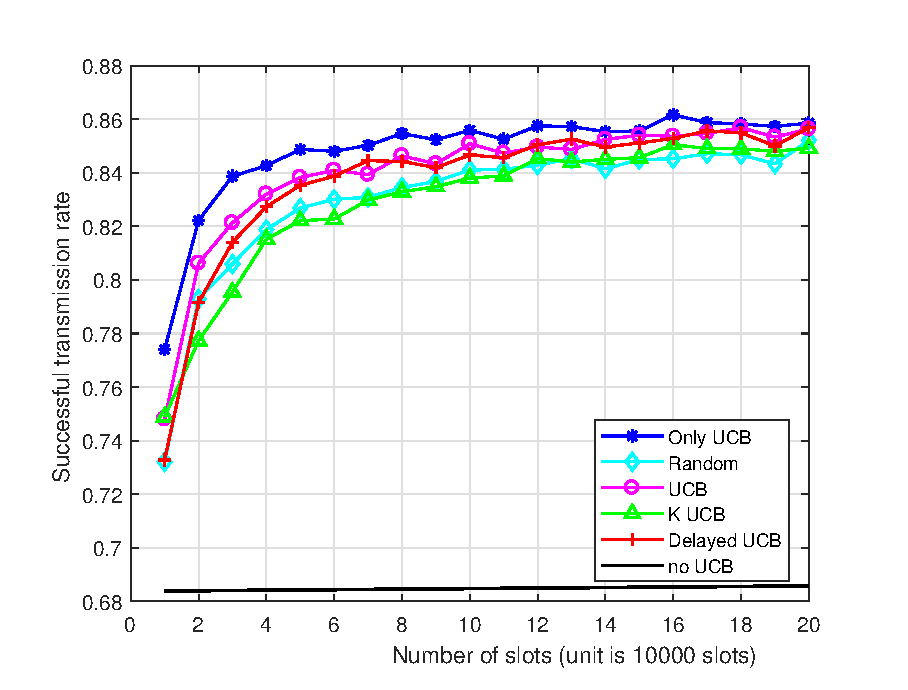
\includegraphics[width=0.80\linewidth]{ResultsUCB.eps}
	\caption[First comparison between the exposed heuristics for the retransmission: ``Only \UCB'', ``Random, \UCB'', ``$K$ \UCB'', and ``Delayed \UCB''.]{
		Comparison between the exposed heuristics for the retransmission:`` \textcolor{blue}{Only \UCB}'', ``\textcolor{cyan}{Random}'', ``\textcolor{purple}{\UCB}'', ``\textcolor{green}{$K$ \UCB}'', and ``\textcolor{red}{Delayed \UCB}''.
		The usage of the same learning policy for transmissions and retransmission is named ``\textcolor{blue}{Only \UCB{}}'',
		whereas the usage of a random channel selection, for both transmission and retransmission, is labeled as ``no \UCB{}''.
		First scenario: learning helps but learning to retransmit smartly is not needed, as we observe that the \textcolor{cyan}{random retransmission} heuristic achieves similar performance than the others.
		We considered $N=1000$ static IoT devices, that occupy the $4$ channels in a static way leading to mean occupancy rates of $10\%,30\%,30\%,30\%$.
	}
	\label{fig:43:mainExperiment1}
\end{figure}

We also consider in our experiment the case of an ALOHA protocol using $\mathrm{MaxBackOff}=5$, and $m=10$, a statistic distribution of the devices about $40\%, 30\%, 20\%, 10\%$ for the four channels, and $N=2000$ IoT devices.
The corresponding results are depicted in Figure~\ref{fig:43:mainExperiment2}.
In this case the successful transmission rate is degraded compared with achieved results in Figure~\ref{fig:43:mainExperiment1}.
We can explain this by the fact that we are considering in our network more devices, which increases the collision probability.
It is important to highlight, that the ``Random'' retransmission heuristic shows a poor performance in comparison to the other heuristics, and it can be attributed to the fact that the number of retransmission is increased, and consequently a
learning approach is able to take advantage of it.
Furthermore, the ``\UCB'', ``$K$ \UCB'' and ``Delayed \UCB'' heuristics behave similarly to ``Only \UCB'', after a similar convergence time.

\begin{figure}[h!]  % [htbp]
	\centering
	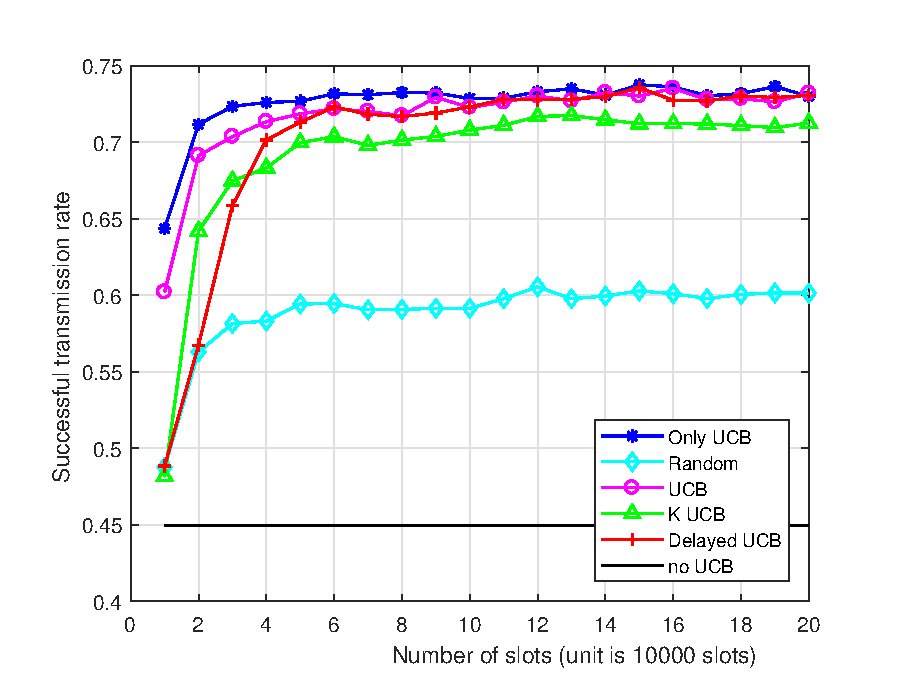
\includegraphics[width=0.80\linewidth]{ResultsUCB2.eps}
	\caption[Second comparison between the exposed heuristics for the retransmission: ``Only \UCB'', ``Random'', ``\UCB'', ``$K$ \UCB'', and ``Delayed \UCB''.]{
		Second scenario: learning helps a lot (a gain of $30\%$ in terms of collision probability), and learning to retransmit smartly is needed.
		We observe that the \textcolor{cyan}{random retransmission} achieves poor performance compared to the others.
		We considered $N=2000$ static IoT devices, that occupy the $4$ channels in a static way leading to mean occupancy rates of $10\%,30\%,30\%,30\%$.
	}
	\label{fig:43:mainExperiment2}
\end{figure}

The conclusions we can draw from these results are twofold.
Firstly, MAB learning algorithms are very useful to reduce the collision rate in LPWA networks, a gain of up-to $30\%$ of successful transmission rate is observed after convergence.
Secondly, using learning mechanisms for retransmissions can be a simple yet efficient and interesting way to reduce collisions in IoT networks, even in networks with massive deployments of IoT as this can be checked in Figure~\ref{fig:43:mainExperiment2}, where the random retransmission heuristic is greatly outperformed by the any of the \UCB-based approaches, that use learning for channel selection during the retransmission procedure.
With $10\%$ to $30\%$ occupancy rates the considered example of IoT network can indeed be considered as an IoT network with a massive deployment of devices.


% \paragraph{Note on the simulation code.}
\paragraph{Reproducibility.}
%
The source code (MATLAB or Octave) used for the simulations and the figures of this section is open-sourced under the MIT License.
It was written in collaboration with Rémi Bonnefoi and Julio César Mango-Vasquez, in the summer $2018$,
and is published at \href{https://Bitbucket.org/scee_ietr/ucb_smart_retrans}{\texttt{Bitbucket.org/scee\_ietr/ucb\_smart\_retrans}}.
